
\paragrafo{No fluxo descrito na seção anterior já é possível encontrar alguns
conceitos SOLID sendo implementados na aplicação web. Porém, será necessário ver
outros fluxos para obter exemplos de implementação que sigam todos os
princípios.}

\begin{subsecao}{Implementação do \acs{SRP}}\label{subsec:dev_srp}

\paragrafo{O Princípio da Responsabilidade Única (\acs{SRP}) está sendo seguido
na classe ShowGameService (Código \ref{alg:showgameservice}). Isso ocorre 
pois a classe tem apenas um propósito, que é a exibição dos detalhes do jogo. 
Sendo assim, a mesma tem um escopo mais restrito em razões para se necessitar 
de alteração, por exemplo, adicionar validações, passar a buscar os jogos pelo 
nome em vez do id, entre outros.}

\vspace{5mm}
\begin{lstlisting}[language=JavaScript, caption={ShowGameService.ts},captionpos=b, label=alg:showgameservice]
import AppError from '@shared/errors/AppError';
import log from '@shared/utils/log';
import { injectable, inject } from 'tsyringe';
import Game from '../infra/typeorm/entities/Game';

import IGamesRepository from '../repositories/IGamesRepository';

interface IRequest {
  game_id: string;
}

@injectable()
export default class ShowGameService {
  constructor(
    @inject('GamesRepository')
    private gamesRepository: IGamesRepository,
  ) {}

  public async execute({ game_id }: IRequest): Promise<Game> {
    log.debug(`Show Game :: id: ${game_id}`);
    const game = await this.gamesRepository.findById(game_id);
    if (!game) {
      throw new AppError('Game not found', 404);
    }
    return game;
  }
}
\end{lstlisting}
\vspace{5mm}
  
\paragrafo{Uma forma fácil de imaginar a classe acima ferindo este princípio
seria se a mesma além de exibir jogos, também criasse ou atualizasse os mesmos.
Com isso, a manutenção dessa classe pode ser mais difícil de se realizar do que
a da primeira:}

\vspace{5mm}
\begin{lstlisting}[language=JavaScript, caption={Implementação que viola o SRP},captionpos=b, label=alg:gameservice]
@injectable()
export default class GameService {
  constructor(
    @inject('GamesRepository')
    private gamesRepository: IGamesRepository,
  ) {}
  public async showGame(data: IShowGameDTO): Promise<Game> {
    //validacoes e processos para exibir detalhes de um jogo
  }
  public async createGame(data: ICreateGameDTO): Promise<Game> {
    //validacoes e processos para criar um jogo
  }
  public async updateGame(data : IUpdateGameDTO): Promise<Game> {
    //validacoes e processos para atualizar um jogo
  }
}
\end{lstlisting}
\vspace{5mm}

\paragrafo{Ao absorver muitas responsabilidades, a classe GameService (Código 
\ref{alg:gameservice}) passa a englobar diversos comportamentos e, com 
isso, passa a exigir mais esforço para se manusear.}

\paragrafo{Uma forma que respeite o \acs{SRP} e implemente as funcionalidades 
da classe GameService pode ser descrita na Figura \ref{fig:srp_example}: Três classes, cada uma 
com suas regras de negócio e suas responsabilidades.}

\begin{figure}[!h]
  \centering
  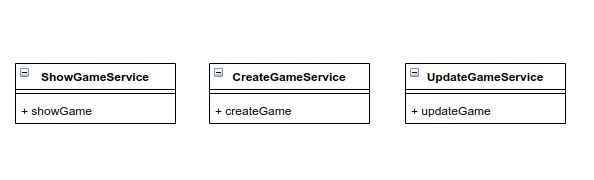
\includegraphics[scale=0.8]{srp_example}
  \caption{Representação do SRP}
  \label{fig:srp_example}
\end{figure}

\paragrafo{Desta forma, o leitor pode se questionar porque a classe
GamesController (Código \ref{alg:gamescontroller}) não viola o \acs{SRP}, visto que 
a mesma realiza todas essas operações. Isso não se caracteriza como uma 
violação pois a responsabilidade da classe é apenas comunicar as chamadas 
recebidas via HTTP para a aplicação. O \emph{Controller} desconhece os 
fluxos de exibição, criação ou atualização, mas conhece as classes 
que contêm esses fluxos.}
\end{subsecao}

\begin{subsecao}{Implementação do \acs{OCP}}\label{subsec:dev_ocp}

\paragrafo{Para exemplificar o Princípio Aberto Fechado (\acs{OCP}), usaremos o
fluxo responsável pela reinvidicação de cartões pré-pagos. Para usar esse
serviço, o usuário insere o código de cartão um cartão pré-pago e resgata jogos
ou dinheiro para a compra de jogos na loja.} 

\paragrafo{Porém, ao cadastrar esses códigos no sistema, a validação para esses
dois tipos de items a ser reinvidicados é diferente. Os cartões de dinheiro
devem resgatar somente os valores de R\$30, R\$50 ou R\$100. Para validar um
jogo, somente é necessário que este exista na base de dados.}

\paragrafo{Com os requisitos acima, um desenvolvedor pode pensar em criar a 
classe descrita no Código \ref{alg:createcodeservice}:}

\vspace{5mm}
\begin{lstlisting}[language=JavaScript, caption={CreateCodeService.ts},captionpos=b, label=alg:createcodeservice]
import { injectable, inject } from 'tsyringe';
import { v4 as uuidv4 } from 'uuid';

import AppError from '@shared/errors/AppError';
import IGamesRepository from '@modules/games/repositories/IGamesRepository';
import IGamestoreCodesRepository from '../repositories/IGamestoreCodeRepository';
import GamestoreCode from '../infra/typeorm/entities/GamestoreCode';

interface IRequest {
  cash?: number;
  game_id?: string;
}

@injectable()
export default class CreateCodeService {
  constructor(
    @inject('GamestoreCodesRepository')
    private gamestoreCodesRepository: IGamestoreCodesRepository,

    @inject('GamesRepository')
    private gamesRepository: IGamesRepository,
  ) {}

  public async execute(request: IRequest): Promise<GamestoreCode | undefined> {
    let code;
    const { cash, game_id } = request;

    if (!cash && !game_id) {
      throw new AppError('Internal Server Error', 500);
    }

    if (cash) {
      if (cash !== 30 && cash !== 50 && cash !== 100) {
        throw new AppError('Invalid cash quantity');
      }

      code = await this.gamestoreCodesRepository.create({
        code: uuidv4(),
        is_redeemed: false,
        product: {
          cash,
        },
      } as GamestoreCode);
    }

    if (game_id) {
      if (!(await this.gamesRepository.findById(game_id))) {
        throw new AppError('Game does not exist');
      }

      code = await this.gamestoreCodesRepository.create({
        code: uuidv4(),
        is_redeemed: false,
        product: {
          game: game_id,
        },
      } as GamestoreCode);
    }
    return code;
  }
}

\end{lstlisting}
\vspace{5mm}

\paragrafo{Embora atenda a demanda, essa estratégia fere o \acs{OCP}. Note que,
se em algum momento no futuro for necessário reinvidicar um terceiro item,
teremos que adicionar mais um if ao método principal dessa classe, o que deixará
o código ainda mais acoplado.} 

\paragrafo{Para ilustrar isso, suponhamos que será necessário reinvidicar
códigos que resgatem Pacotes de Expansão para jogos já cadastrados em nossa
plataforma. Essa funcionalidade extrapola o escopo desse trabalho, mas sua
implementação pode ser descrita no código \ref{alg:ocpviolation}.}

\vspace{5mm}
\begin{lstlisting}[language=JavaScript, caption={Implementação que viola o OCP},captionpos=b, label=alg:ocpviolation]
interface IRequest {
  cash?: number;
  game_id?: string;
  dlc_id?: string;
}

@injectable()
export default class CreateCodeService {
  constructor(
    @inject('GamestoreCodesRepository')
    private gamestoreCodesRepository: IGamestoreCodesRepository,

    @inject('GamesRepository')
    private gamesRepository: IGamesRepository,

    @inject('DlcsRepository')
    private dlcsRepository: IDlcsRepository,
  ) {}

  public async execute(request: IRequest): Promise<GamestoreCode | undefined> {
    if (!request.cash && !request.game_id && !request.dlc_id) {
      throw new AppError('Internal Server Error', 500);
    }

    if (request.cash) {
      //validacao de cash (R$30, R$50 ou R$100)
      //cadastro do cartao pre pago de cash
    }

    if (request.game_id) {
      //validacao de game (se o game existe)
      //cadastro do cartao pre pago de gane
    }

    if (request.dlc_id) {
      //validacao de dlc (se a dlc existe)
      //cadastro do cartao pre pago de gane
    }
  }
}
\end{lstlisting}
\vspace{5mm}

\paragrafo{Para não ferir este princípio, basta estendermos a funcionalidade de
uma classe base e realizar as validações nas classes herdeiras. A seguir temos
os passos para realizar esse procedimento:} 

\paragrafo{Primeiramente, definimos uma classe abstrata (Código 
\ref{alg:abstractcode}) que concentrará os métodos que serão realizados pelas
classes filhas desta. Como os fluxos de cadastro de códigos para jogo e dinheiro
virtual passam por processos diferentes de validação e cadastro, este serão 
métodos abstratos desta classe.}

\vspace{5mm}
\begin{lstlisting}[language=JavaScript, caption={Classe Abstrata},captionpos=b, label=alg:abstractcode]
  export default abstract class AbstractCodeTemplate {
    public async execute(request: IRequest): Promise<GamestoreCode> {
      await this.validateData(request);
      const code = await this.createCode(request);
      return code;
    }
  
    protected abstract createCode(request: IRequest): Promise<GamestoreCode>;
    protected abstract validateData(request: IRequest): Promise<void>;
  }
\end{lstlisting}  
\vspace{5mm}

\paragrafo{Em seguida, estendemos, a partir da classe abstrata, uma classe para
cada comportamento diferente. Sendo assim, uma classe para validar e registrar
jogos (Código \ref{alg:gamecodeservice}) e outra para dinheiro virtual 
(Código \ref{alg:cashcodeservice}).}

\begin{figure}[!h]
  \centering
  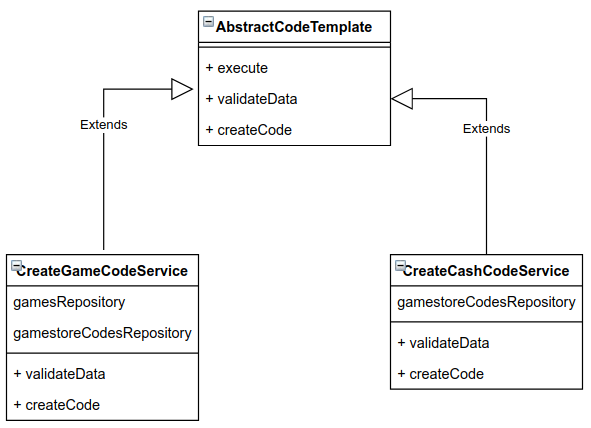
\includegraphics[scale=0.75]{ocp_example}
  \caption{Representação do OCP}
  \label{fig:ocp_example}
\end{figure}

\paragrafo{Na Figura \ref{fig:ocp_example},
temos uma representação de como essas classes se relacionam. As setas 
partem em direção a classe abstrata, indicando a classe que estende a mesma.}

\vspace{5mm}
\begin{lstlisting}[language=JavaScript, caption={Cadastro de Códigos para Jogos},captionpos=b, label=alg:ocpexample]
interface IRequest {
  game_id: string;
}

@injectable()
export default class CreateGameCodeService extends AbstractCodeTemplate {
  constructor(
    @inject('GamesRepository')
    private gamesRepository: IGamesRepository,

    @inject('GamestoreCodesRepository')
    private gamestoreCodesRepository: IGamestoreCodesRepository,
  ) {
    super();
  }

  protected async createCode({ game_id }: IRequest): Promise<GamestoreCode> {
    //cria codigo para o jogo
  }

  protected async validateData({ game_id }: IRequest): Promise<void> {
    if (!validateUuid(game_id) || !(await this.gamesRepository.findById(game_id))) {
      throw new AppError('Game does not exist');
    }
  }
}
\end{lstlisting}
\vspace{5mm}

\vspace{5mm}
\begin{lstlisting}[language=JavaScript, caption={Cadastro de Códigos para Dinheiro Virtual},captionpos=b, label=alg:cashcodeservice]
@injectable()
export default class CreateCashCodeService extends AbstractCodeTemplate {
  constructor(
    @inject('GamestoreCodesRepository')
    private gamestoreCodesRepository: IGamestoreCodesRepository,
  ) {
    super();
  }

  protected async createCode(data: IRequest): Promise<GamestoreCode> {
    const code = await this.gamestoreCodesRepository.create(/*
      dados do dinheiro virtual
    */);
    return code;
  }

  protected async validateData(data: IRequest): Promise<void> {
    //algoritmo de validacao do dinheiro virtual
  }
}
\end{lstlisting}
\vspace{5mm}

\end{subsecao}
\begin{subsecao}{Implementação do \acs{LSP}}\label{subsec:dev_lsp}

\paragrafo{Um bom exemplo de implementação que respeita o LSP já foi apresentado na subseção 
anterior. }

\paragrafo{Esse princípio pode ser quebrado se, por exemplo, a interface não 
especificar um método requerido em algum dos casos de uso e terceirizar essa 
responsabilidade diretamente para as subclasses. A intercambiabilidade é perdida,
e assim, a possibilidade de reuso do código também.}

\paragrafo{O benefício de se usar esse príncipio está na desacoplação do código.
Sem esse princípio aplicado, por exemplo, seria necessário especificar o subtipo
UsersRepository, que, como demonstrado previamente, por se tratar de um 
Adaptador de Interfaces, é um módulo de nível inferior aos Casos de Uso.}

\end{subsecao}

\begin{subsecao}{Implementação do \acs{ISP}}\label{subsec:dev_isp}

\paragrafo{Um exemplo muito recorrente do próximo princípio, isto é, o
Princípio da Segregação de Interfaces (\acs{ISP}), está no funcionamento 
das classes \emph{Repository} da aplicação.} 

\vspace{5mm}
\begin{lstlisting}[language=JavaScript, caption={Interace a ser implementada},captionpos=b, label=alg:iusersrepository]
import ICreateUserDTO from '../dtos/ICreateUserDTO';
import User from '../infra/typeorm/entities/User';

export default interface IUsersRepository {
  findById(id: string): Promise<User | undefined>;
  findByEmail(email: string): Promise<User | undefined>;
  create(data: ICreateUserDTO): Promise<User>;
  save(user: User): Promise<User>;
}
\end{lstlisting}
\vspace{5mm}

\paragrafo{Tomando por exemplo o \emph{Repository} de Usuários,
temos a interface IUsersRepository (Código \ref{alg:iusersrepository})
e suas implementações UsersRepository (Código \ref{alg:usersrepository})
e FakeUsersRepository (Código \ref{alg:fakeusersrepository}).}

\vspace{5mm}
\begin{lstlisting}[language=JavaScript, caption={UsersRepository.ts},captionpos=b, label=alg:usersrepository]
import { getRepository, Repository } from 'typeorm';
import IUsersRepository from '@modules/users/repositories/IUsersRepository';

import ICreateUserDTO from '@modules/users/dtos/ICreateUserDTO';
import log from '@shared/utils/log';
import User from '../entities/User';

class UsersRepository implements IUsersRepository {
  private ormRepository: Repository<User>;

  constructor() {
    this.ormRepository = getRepository(User);
  }

  public async findById(id: string): Promise<User | undefined> {
    log.debug('Users :: findById');
    return this.ormRepository.findOne(id);
  }

  public async findByEmail(email: string): Promise<User | undefined> {
    log.debug('Users :: findByEmail');
    const user = await this.ormRepository.findOne({
      where: { email },
    });
    return user;
  }

  public async create(userData: ICreateUserDTO): Promise<User> {
    log.debug('Users :: create');
    const user = this.ormRepository.create(userData);
    await this.ormRepository.save(user);
    return user;
  }

  public async save(user: User): Promise<User> {
    log.debug('Users :: save');
    return this.ormRepository.save(user);
  }
}

export default UsersRepository;
\end{lstlisting}
\vspace{5mm}

\paragrafo{Podemos dizer que o \acs{ISP} é respeitado na relação entre esses
três módulos pois a interface IUsersRepository tem 100\% dos seus métodos usados 
por suas implementações.} 

\vspace{5mm}
\begin{lstlisting}[language=JavaScript, caption={FakeUsersRepository.ts},captionpos=b, label=alg:fakeusersrepository]
import IUsersRepository from '@modules/users/repositories/IUsersRepository';
import ICreateUserDTO from '@modules/users/dtos/ICreateUserDTO';

import { v4 as uuidv4 } from 'uuid';
import User from '../../../../modules/users/infra/typeorm/entities/User';

export default class FakeUsersRepository implements IUsersRepository {
  private users: User[] = [];

  public async findById(id: string): Promise<User | undefined> {
    return this.users.find(user => user.id === id);
  }

  public async findByEmail(email: string): Promise<User | undefined> {
    return this.users.find(user => user.email === email);
  }

  public async create(userData: ICreateUserDTO): Promise<User> {
    const user = new User();
    Object.assign(user, { id: uuidv4() }, userData);
    this.users.push(user);
    return user;
  }

  public async save(user: User): Promise<User> {
    const findIndex = this.users.findIndex(findUser => findUser.id === user.id);
    this.users[findIndex] = user;
    return user;
  }
}
\end{lstlisting}
\vspace{5mm}

\paragrafo{Na Figura \ref{fig:isp_example}, temos a representação gráfica de como 
os módulos citados se relacionam e como eles constituem o \acs{ISP}. As setas 
tracejadas representam a implementação da interface IUsersRepository.}

\begin{figure}[!h]
  \centering
  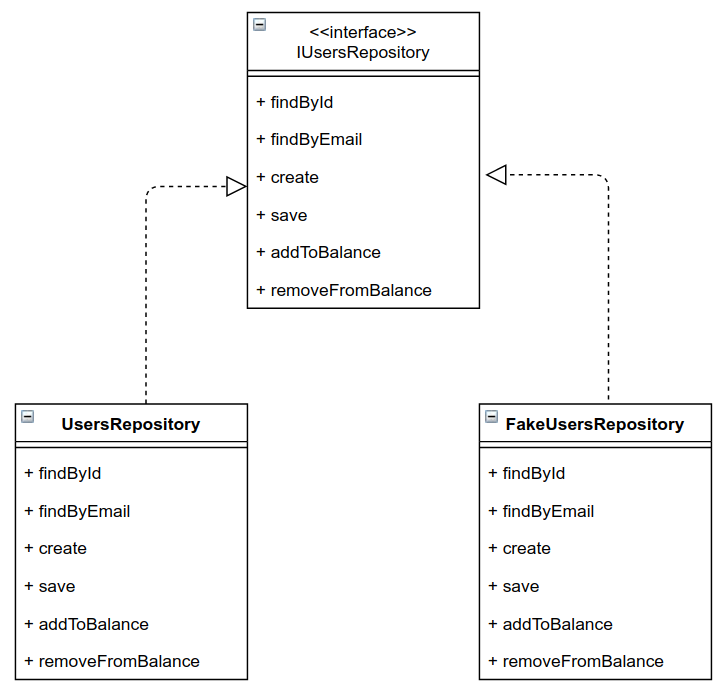
\includegraphics[scale=0.6]{isp_example}
  \caption{Representação do ISP}
  \label{fig:isp_example}
\end{figure}

\paragrafo{Esse princípio pode ser quebrado se, como exemplificado na Seção 
\ref{subsec:ISP}, a interface especificar um método que uma de suas implementações
não necessite. Ao fazer isso, perde-se os benefícios que uma abstração de interfaces
pode promover, como o reuso do código.}

\paragrafo{O benefício de se usar esse príncipio está na desacoplação do código.
Sem esse princípio aplicado, por exemplo, seria necessário especificar o subtipo
UsersRepository, que, como demonstrado previamente, por se tratar de um 
Adaptador de Interfaces, é um módulo de nível inferior aos Casos de Uso.}

\end{subsecao}

\begin{subsecao}{Implementação do \acs{DIP}}\label{subsec:dev_dip}

\paragrafo{A aplicação do Princípio da Inversão de Dependência pode ser encontrada
em todos os Casos de Uso da aplicação que interajam com o banco de dados, visto
que todos eles importam a dependência a partir de uma abstração. A Figura 
\ref{fig:dip_example} ilustra essa situação com classes que já foram apresentadas
previamente.}

\begin{figure}[!h]
  \centering
  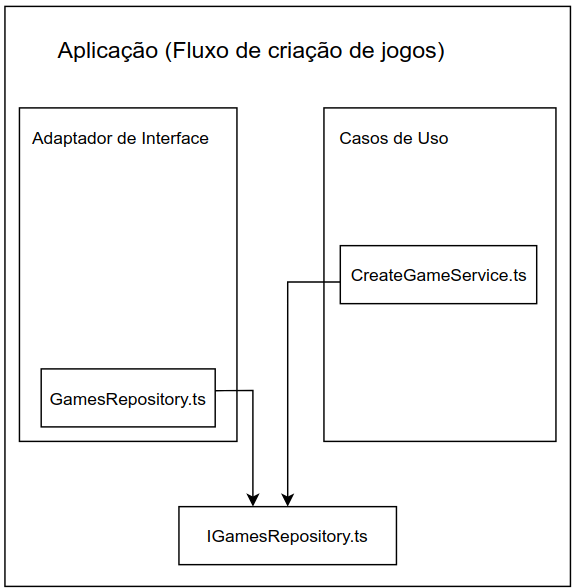
\includegraphics[scale=0.5]{dip_example}
  \caption{Representação do DIP}
  \label{fig:dip_example}
\end{figure}

\paragrafo{Para visualizar um modelo que viole a implementação do \acs{DIP}, basta
fazer que o Caso de Uso CreateGameService importe diretamente a dependência
GamesRepository, como exemplificado através do Código \ref{alg:dip_violation} 
e da Figura \ref{fig:dip_violation}.} 

\vspace{5mm}
\begin{lstlisting}[language=JavaScript, caption={O Caso de Uso},captionpos=b, label=alg:dip_violation]
  export default class CreateGameService {
    constructor(
      private gamesRepository: new GamesRepository(),
    ) {}
  
    public async execute(data: ICreateGameDTO): Promise<Game> {
      //validacoes
      return await this.gamesRepository.create(/* dados do jogo */);
    }
  }
\end{lstlisting}

\vspace{5mm}

\begin{figure}[!h]
  \centering
  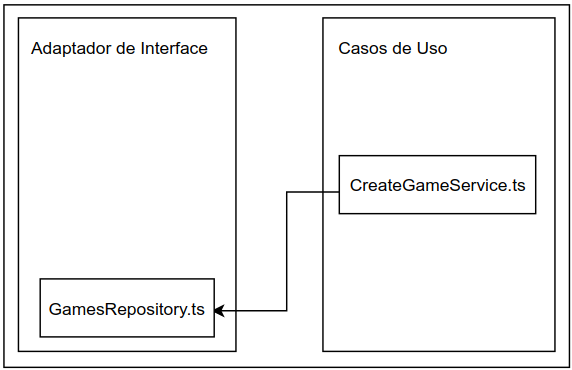
\includegraphics[scale=0.75]{dip_violation}
  \caption{Violação do DIP}
  \label{fig:dip_violation}
\end{figure}

\end{subsecao}

\begin{subsecao}{Benefícios do SOLID}\label{subsec:solid_benefits}
\paragrafo{Com isso, podemos refletir sobre os benefícios da aplicação 
desses princípios. O \acs{SRP} e o \acs{OCP}, por exemplo, garantem 
a facilidade de leitura e entendimento do código ao separar funcionalidades 
complexas em componentes menores.}
\paragrafo{O \acs{LSP} e o \acs{ISP} exploram e determinam regras para o uso do 
conceito de interface e herança de forma a garantir a coesão do código e que 
boas abstrações sejam construídas.}
\paragrafo{O \acs{DIP} permite que módulos de nível superior possam referenciar, 
indiretamente, módulos de nível inferior sem acarretar acoplamento entre estes.}
\paragrafo{Por fim, se atentar aos princípios SOLID traz como 
principais benefício, de diferentes formas, um código mais manuseável e limpo, 
menos suscetível a bugs inesperados e com maior potencial de crescimento00.}
\end{subsecao}